\section{Introducción}
Dentro de las fases para el desarrollo de un proyecto de minería de datos, después del entendimiento del dominio, se encuentra el entendimiento de los datos. Este capítulo se enmarca en el entendimiento de los datos y describe los resultados producto de las dos tareas siguientes: (1) descripción de la lista de problemas desde cada una de las dimensiones de estudio (paciente, fecha de registro, problema cargado, área jerárquica del especialista, grupo etario del paciente y nivel de asistencia) y (2) construcción de grupos de problemas según el contexto. 

La primera tarea permite determinar la calidad de los datos y definir los criterios para la construcción del conjunto de entrenamiento y validación. En la segunda tarea se crean los \textit{\acrshort{refset}} que pueden ser utilizados como vocabularios controlados dependientes de contextos. Estas tareas  tienen el objetivo de reducir la cardinalidad de algunas de las dimensiones mencionadas y permitir la interoperabilidad de los datos y de esta manera facilitar su posterior comparación con los realizados en otras instituciones.

\section{Comprensión de datos}
La lista de problemas registra las observaciones y hallazgos realizados a los pacientes y otra información del contexto. Los problemas de los pacientes son descripciones que se agrupan en conceptos, y los conceptos a su vez pertenecen a uno o varios \textit{\acrshort{refset}}.

Cualquier usuario con acceso a la \acrshort{HCE} puede registrar un problema, este usuario puede pertenecer a una área administrativa o asistencial del \acrshort{HIBA}. Algunas de las áreas tienen sub-áreas, presentando así una estructura jerárquica. Cuando se registra un problema, se asocia el área jerárquica del que registra.

Además cada registro tiene el atributo nivel de asistencia que indica el ámbito en el que fue cargado el problema (1 = Ambulatorio , 2 = Internacion General, 3 = Guardia, 4 = Triage, 5 = Internacion Geriatrica, 6 = Internacion Domiciliaria, 7 = Seguimiento Domiciliario, 8 = Episodio Externo, 9 = Episodio Ambulatorio). La figura \ref{fig:ModeloER} contiene el modelo entidad relación, donde se muestra cómo se relacionan estos datos.

\begin{figure}[htbp]
\caption{Modelo Entidad-Relación de lista de problemas}
\label{fig:ModeloER}
\centering
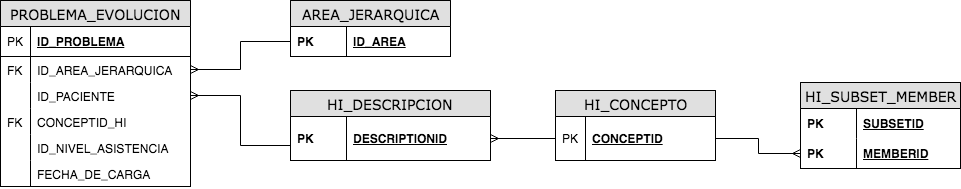
\includegraphics[width=0.9\textwidth]{ER_Problemas}
\end{figure}

 A continuación describo la distribución de los problemas para cada una de las dimensiones de la entidad PROBLEMA\_EVOLUCION.
 
\subsection{Distribución en el tiempo}
El atributo FECHA\_DE\_CARGA indica la fecha en la que se cargó el problema por primera vez. Para las anotaciones posteriores se vuelve a usar el problema registrado y no se crea uno nuevo. En la figura \ref{fig:registrosYConceptos}, se puede observar que aunque la implementación de la \acrshort{HCE} empezó en el año 1998, hay registros anteriores a esa fecha, los cuales se interpretan como errores en el momento de la carga, al igual que los registros con las fechas superiores al 2017. En total son \num{9149} casos que corresponden al \num{0,004}\% de los datos.

Como se muestra en la figura \ref{fig:registrosYConceptos} la distribución no es uniforme, su crecimiento se explica por los hitos de implementación dentro de la HC, en el año \num{2002} se generalizó el uso de la HCE en todo el hospital, y en el año \num{2006} se implementó el servidor de terminología. Los años \num{2015} y \num{2016} muestran un incremento en el registro de la lista de problemas.

En cuanto a los conceptos diferentes registrados por año, se observa una distribución más uniforme, especialmente después del año \num{2007}. Los datos del año 2017 son sólo los del primer semestre.

\begin{figure}[htbp]
\caption{Distribución de problemas por año de carga}
\label{fig:registrosYConceptos}
\centering
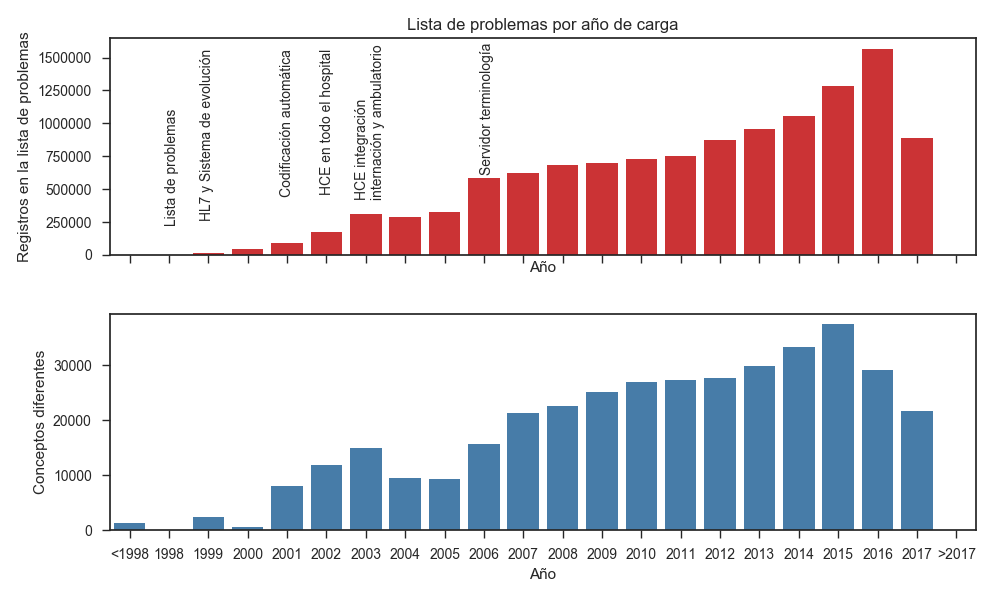
\includegraphics[width=\textwidth]{chart1}
\end{figure}

\subsection{Distribución por paciente (individuo)}
Según la figura \ref{fig:listaIndividuos} la mayoría de los individuos tiene sólo un problema registrado en su lista de problemas, estos corresponde al \num{34.1}\% de los datos. Los individuos que tienen registrados hasta 10 problemas en la lista son el \num{80}\% de los datos.

\begin{figure}[htbp]
\caption{Distribución del tamaño de la lista de problemas por individuos}
\label{fig:listaIndividuos}
\centering
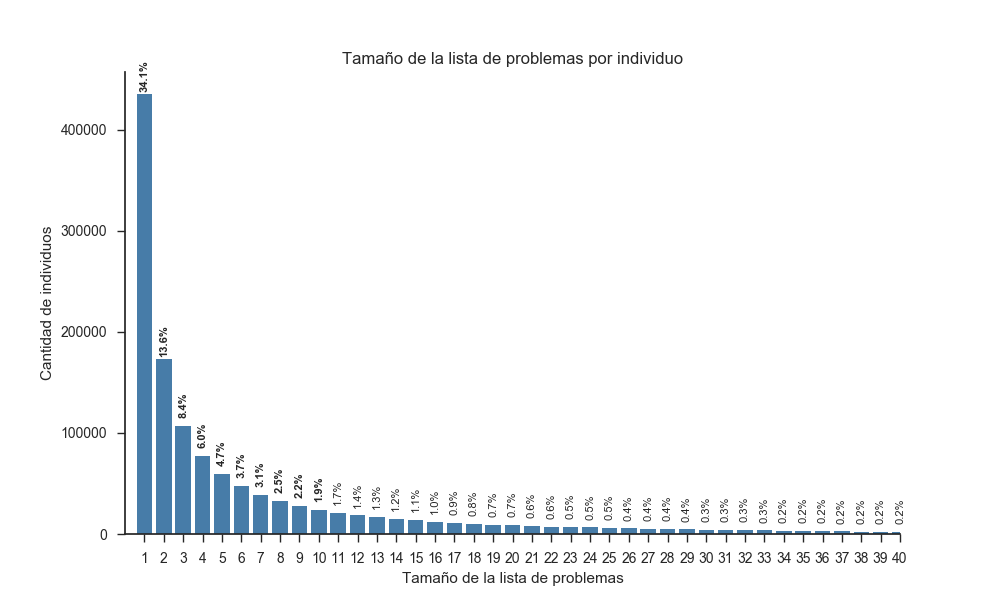
\includegraphics[width=\textwidth]{chart2}
\end{figure}

\subsection{Distribución por conceptos}
El conjunto de datos contiene \num{88869} conceptos distintos usados para identificar problemas de los pacientes. La figura \ref{fig:listaProblemas} representa el uso de estos conceptos en todos los registros de la lista de problemas, en ella se observa que un conjunto pequeño de problemas tiene una frecuencia muy alta y el resto que queda en la cola de la distribución fueron usados muy pocas veces. Los conceptos con más frecuencia de uso son Control de salud, Fiebre, Dolor abdominal,  Hipertensión arterial, Catarro de las vías áreas superiores, Malestar general, Tos, Embarazo, Lumbalgia, Broncoespasmo, Evaluación inicial del paciente e Infección del tracto urinario. Juntos estos trastornos representan el \num{20}\% del total de registros. 

\begin{figure}[htbp]
\caption{Distribución de todos los problema por su aparición en la lista}
\label{fig:listaProblemas}
\centering
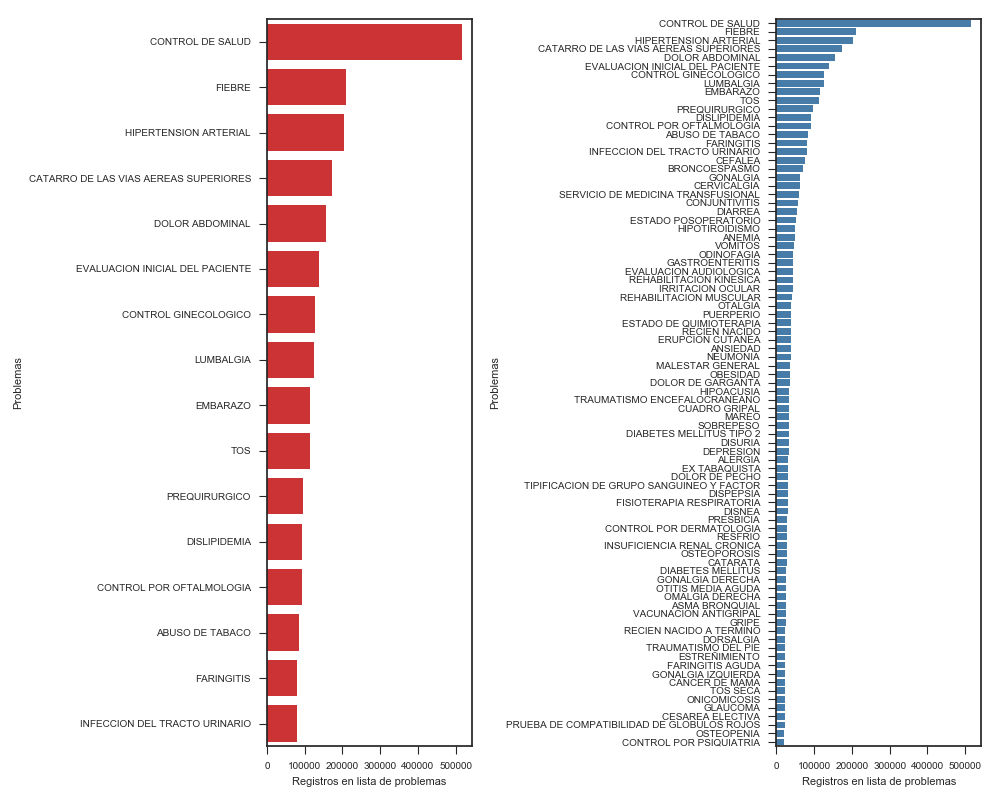
\includegraphics[width=\textwidth]{chart3}
\end{figure}

\subsection{Distribución por contextos}

Los contextos que tuve en cuenta en esta tesis fueron área jerárquica, nivel de asistencia y grupo etario, a continuación describo cómo se distribuyen los conceptos y registros de la lista de problemas en los contextos.


\subsubsection{Contexto: Nivel de asistencia}
%%Los niveles de asistencia son las diferentes modalidades de contacto que tiene el paciente con el hospital, asegurando una óptima atención en cada situación específica. En la \acrshort{HCE} el nivel de asistencia puede ser cualquier de los siguientes valores:

% \begin{itemize}
% \item Ambulatorio: Se tiene definido cuándo empieza y cuándo termina  esa atención. El paciente solicita previamente un turno ambulatorio.
% \item Episodio ambulatorio: Se sabe cuándo empieza pero no cuándo termina; entonces la modalidad de registro cambia. En el ambulatorio generalmente hay alguien que longitudinalmente ve al paciente en distintos momentos.
% \item Triage: Se genera cuando un paciente tiene un contacto con el hospital sin un turno previo, consiste en una revisión médica rápida que permite definir la prioridad de atención.
% \item Guardia: Los pacientes críticos con inminencia de muerte o que ingresa con una patología aguda, de gravedad moderada o severa, pero sin muerte inminente por la misma. En este nivel de asistencia se espera que el alta del nivel se dé entre las 24 y 36 horas de su ingreso, pudiendo trasladarse a otro nivel asistencial del hospital, o a otro hospital, o más rara vez a su domicilio.
% \item Internación: Tiene un periodo limitado del cuidado, el paciente es tratado por un episodio grave de una enfermedad, cuyas condiciones puedan resultar en un trauma o su muerte. Los tipos de internación son general, domiciliaria y geriátrica.
% \end{itemize}

Según la tabla \ref{nivel_asistencia} se puede observar que en cuatro niveles de asistencia (Ambulatorio, Guardia, Triage e Internación general (Ver sección \ref{par:listaproblemas-HCE})) están el 97\% del total de los registros de la lista de problemas. De estos cuatro niveles de asistencia, en el caso de Ambulatoria por cada 81 registros hay un concepto de Snomed CT diferente asociado a la lista de problemas, en la guardia esta relación es de 105:1. Triage es la relación más baja ya que es 188:1 entre los registros y los conceptos de Snomed  CT, e Internación General es la más alta (42:1).

\begin{table}[tb]
\centering
\caption{Distribución de registros y conceptos por nivel de asistencia o ámbito }
\label{nivel_asistencia}
\begin{tabular}{@{}lrr@{}}
\toprule
Nivel de Asistencia o ámbito & Registros & Diferentes Conceptos \\ \midrule
Ambulatorio & \num{771096} & \num{9543} \\
Guardia & \num{603412} & \num{5759} \\
Triage & \num{556166} & \num{2963} \\
Internación general & \num{267303} & \num{6322} \\
Internación domiciliaria & \num{22297} & \num{1975}\\
Episodio ambulatorio & \num{17947} & \num{1247} \\
Seguimiento domiciliario & \num{14537} & \num{1302} \\
Internación geriátrica & \num{204} & \num{115} \\ \bottomrule
\end{tabular}
\end{table}

\subsubsection{Contexto: Grupo etario}
La distribución de los problemas registrados por edad en la figura \ref{fig:listaEdad} evidencia que los grupos etarios en los que más se consulta son 0-4 años, 25-34 años y mayores de 75 años.

\begin{figure}[htbp]
\caption{Distribución de todos los problema por edad de los pacientes}
\label{fig:listaEdad}
\centering
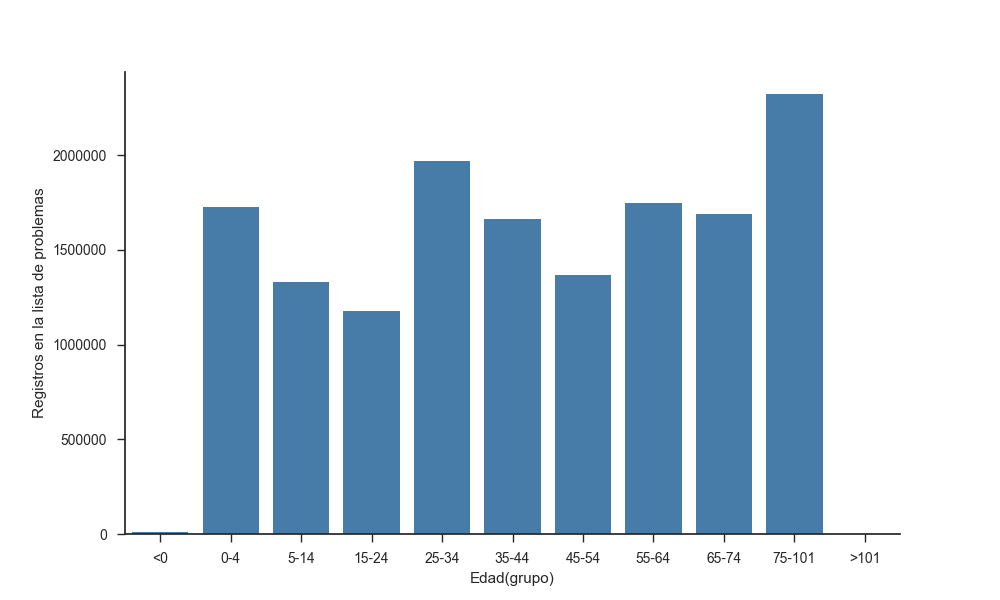
\includegraphics[width=\textwidth]{chart4}
\end{figure}

\subsubsection{Contexto: Área Jerárquica}
La \acrshort{HCE} tiene 918 áreas jerárquicas, de las cuales 601 tienen usuarios que han registraron problemas dentro de la lista de algún paciente. Hay ocho jerarquías que usan más de \num{10000} conceptos (Clínica médica y Medicina Familiar, Traumatología y ortopedia, Clínica pediátrica, Departamento de enfermería, Central de emergencia de adultos, Cirugía general y Dermatología), el resto de jerarquías usan en promedio menos de \num{5000} conceptos. (Ver figura \ref{fig:listaArea}).  En la siguiente sección, que corresponde a la creación de los contextos, se evalúa si los datos de la lista de problemas necesitan también de ese nivel de detalle, o si las áreas pueden ser agrupadas.

\begin{figure}[htbp]
\caption{Registros y conceptos únicos en las top 50 áreas jerárquicas.}
\label{fig:listaArea}
\centering
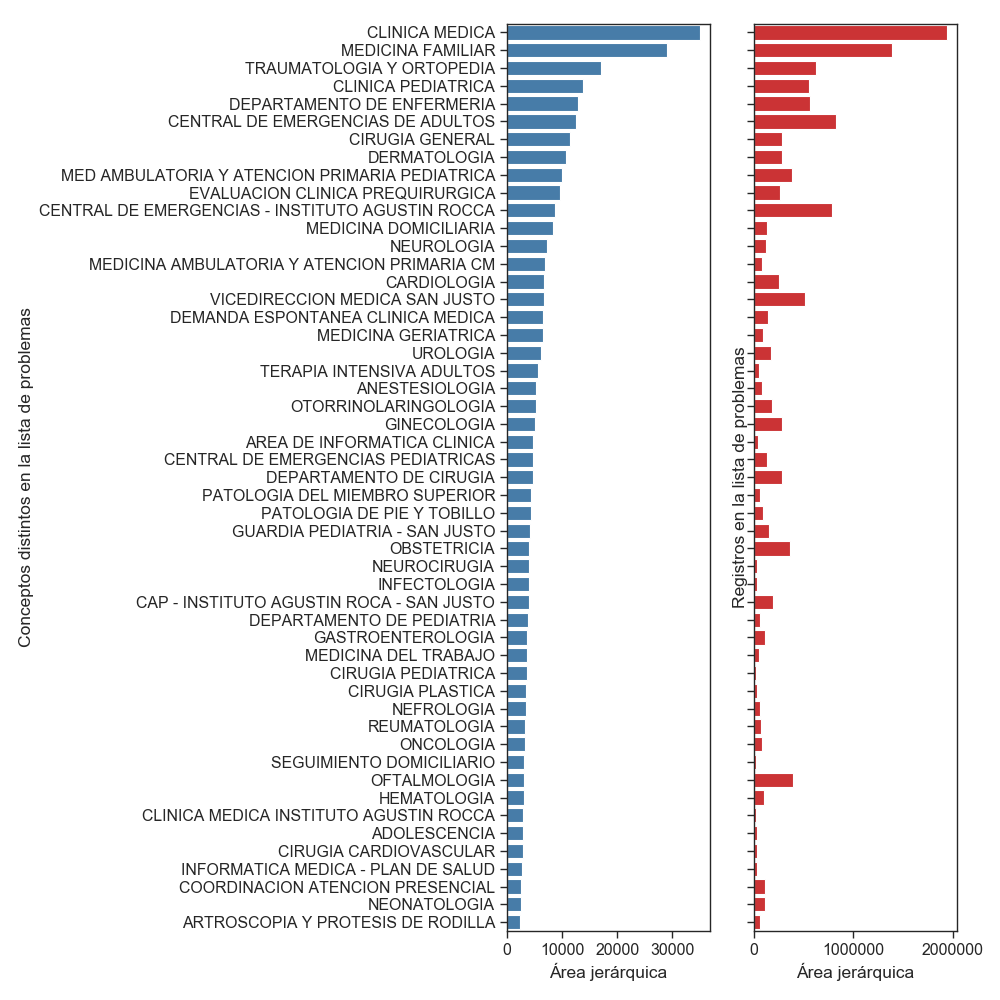
\includegraphics[width=\textwidth]{chart5}
\end{figure}

% Las áreas jerárquicas que tiene el \acrshort{HIBA} responden a necesidades operativas de la \acrshort{HCE}, y tienen diferentes niveles de agregación, por ejemplo: Sección de neurocirugía vascular hace parte de una área más general llamada Servicio de neurocirugía. También existen áreas jerárquicas con muy pocos conceptos o que son \textit{ad hoc} por ejemplo: Instituto universitario H.I., Programa de prevención del cáncer de colon hereditario, Laser en rinosinusología. .

\section{\textit{Refsets} según el contexto}

En la primera fase de preparación de los datos, creé la base de datos de grafos. En el modelo de datos que se observa a la izquierda de la figura \ref{fig:ModeloDatosContexto} los vértices son los \textbf{conceptos} que está relacionados entre si por la arista \textbf{(ES\_UN)}, y los \textbf{contextos} están relacionados con los \textbf{conceptos} con la arista \textbf{(REGISTRA\_PROBLEMA)}, esta relación tiene el atributo \textbf{Frecuencia}. Este modelo representa los diferentes niveles de generalización de los conceptos con la relación (ES\_UN). También se representa que un contexto (área jerárquica, nivel asistencial o grupo etario) tiene varios conceptos y un concepto puede estar en varios contextos con la relación (REGISTRA\_PROBLEMA). A la derecha de la figura  \ref{fig:ModeloDatosContexto} hay una instancia de este modelo. Se representa que contextualmente el concepto varicela está registrado 150 veces en el área jerárquica Pediatría, 20 veces en el nivel asistencial Triage y 10 en el grupo etario de 5 a 14 años. Semánticamente, la varicela es una enfermedad viral caracterizada por exantema y es una infección por virus varicela zoster.

\begin{figure}[htbp]
\caption{Modelo de datos con contexto}
\label{fig:ModeloDatosContexto}
\centering
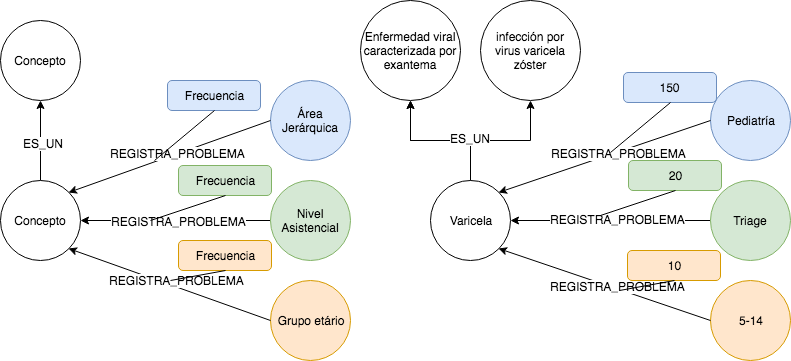
\includegraphics[width=\textwidth]{Modelo_datos_contexto}
\end{figure}

El siguiente paso fue la detección del solapamiento entre los grupos y la posterior generación de los grupos contextuales finales, para realizar este paso se aplicaron algoritmos de aprendizaje no supervisado. A continuación describo los resultados obtenidos por cada uno de los contextos.

\subsection{Contexto: Nivel de asistencia}
Con el fin de encontrar conceptos que estén asociados a los niveles de asistencia apliqué los algoritmos de agrupamiento \textit{leading vector}, \textit{label propagation} y \textit{multilevel} (Ver sección \ref{par:aprendizaje_nosupervisado})). Los valores de modularidad y número de grupos son similares aplicando todos los algoritmos:
\begin{itemize}
\item \textit{Leading vector}: modularidad = \num{0.346}, número de grupos = 4, test: P=0.000
\item \textit{Label propagation}: modularidad = \num{0.393} , número de grupos = 5, test: P=0.000
\item \textit{Multilevel}: modularidad = \num{0.397} , número de grupos = 5, test: P=0.000
\end{itemize}
\footnote{La fase de diseño y evaluación (Sección \ref{par:disenho_evaluacion}) contiene los pasos que se siguieron para realizar los test de signficancia de los \textit{clusters}}

La tabla \ref{nivel_asistencia_clus} contiene los conceptos que se comparten en todos los grupos después de aplicar los algoritmos de agrupamiento. Los niveles de asistencia Internación general e Internación domiciliaria contienen los mismos conceptos. Después de fusionar estos dos niveles, son 3002 conceptos que representan su contexto.

\begin{table}[htb]
\centering
\caption{Contexto de nivel de asistencia y sus conceptos }
\label{nivel_asistencia_clus}
\begin{tabular}{@{}lr@{}}
\toprule
Nivel de Asistencia o ámbito & Conceptos finales del grupo \\ \midrule
Ambulatorio & \num{6304} \\
Guardia & \num{2269} \\
Triage & \num{779} \\
Internación general & \num{3002} \\
Internación domiciliaria  & \num{3002}\\
Episodio ambulatorio & \num{370} \\
Seguimiento domiciliario & \num{681}\\
Internación geriátrica & \num{101} \\ \bottomrule
\end{tabular}
\end{table}


\subsection{Contexto: Grupo etario}
\label{par:contexto-grupo-etario}
Al aplicar los algoritmos de agrupamiento, obtengo resultados similares entre \textit{Leading vector} y \textit{multilevel}. \textit{Leading Vector} dividió el grafo en cinco grupos y la modularidad  fue de \num{0.171}. \textit{Multilevel} dividió el grafo en 4 grupos con una modularidad de \num{0.138}. En el caso del algoritmo \textit{label propagation} el valor de la modularidad es de 0, por lo tanto sus resultados son descartados.

Después de combinar los resultados de los algoritmos \textit{Leading vector} y \textit{multilevel}, para identificar los grupos que invariantemente se repitan en ambos resultados, se descarta el grupo etario de 5 a 14 años y fusionan los grupos etarios de 0 a 4, 15 a 24, 25 a 34 y 35 a 44 años. La tabla \ref{grupo_etario_clus} contiene los tamaños finales de los grupos.


% Please add the following required packages to your document preamble:
% \usepackage{booktabs}
\begin{table}[htb]
\centering
\caption{Contexto del grupo etario  y sus conceptos}
\label{grupo_etario_clus}
\begin{tabular}{@{}lr@{}}
\toprule
Grupo Etario & Conceptos del grupo \\ \midrule
0-4  & \num{12532} \\
5-14 & \num{0} \\
15-24  & \num{12532} \\
25-34  & \num{12532} \\
35-44 & \num{12532} \\
45-54  & \num{6731} \\
55-64  & \num{5073} \\
65-74  & \num{5165} \\
75-101 & \num{4292} \\ \bottomrule
\end{tabular}
\end{table}

\subsection{Contexto: áreas jerárquicas}
\label{par:contexto-areas}
Como se definió en la fase del entendimiento de los datos de la metodología (sección \ref{par:entendimiento_datos}), la creación de los \textit{\acrshort{refset}} de áreas jerárquicas consiste en la ejecución de las 3 tareas siguientes: (1) en la definición de los contextos significativos y (2) identificación de solapamientos entre \textit{\acrshort{refset}} y (3) evaluación final. 

Se define como área significativa las que tienen un mapeo a Snomed CT. Su identificación se realiza con \textit{string matching} de las áreas jerárquicas a  alguno de los descendientes de  los \textbf{servicios de la atención de la salud (SCTID: 224891009)} de SNOMED CT. Si no hay un mapeo, se selecciona el servicio de las áreas que tengan sobreposición en sus conceptos con los \textit{clusters} previamente identificados con el \textit{string matching}. Se excluyen las áreas que tienen un sólo concepto, y las áreas que entran dentro del \textit{cluster} identificado como administrativo. 

\paragraph{Diseño del modelo}: Ejecuté 3 algoritmos de agrupamiento. como se observa en la tabla \ref{clusteringAreas}, el algoritmo \textit{leading vector} dividió el conjunto de datos en 2 y su modularidad es la más baja por lo tanto sus resultados se descartaron.  Los resultados de los otros dos algoritmos se usaron como criterio para seleccionar la jerarquía final.

\begin{table}[htb]
\centering
\caption{Agrupamiento de áreas jerárquicas y conceptos}
\label{clusteringAreas}
\begin{tabular}{@{}llll@{}}
\toprule
Algoritmo         & Modularidad & Grupos & Test \\ \midrule
Label Propagation & 0.165       & 18     &   0.000   \\
Leading Vector    & 0.144       & 2      &     0.000 \\
MultiLevel        & 0.447       & 14     &     0.000 \\ \bottomrule
\end{tabular}
\end{table}

\paragraph{Resultados de contexto significativos}

Ejemplos de los resultados de la aplicación de los criterios de exclusión y de selección del primer experimento se encuentran en la tabla \ref{ejemploCriterios}. Los resultados de la aceptación de estos criterios se encuentran en la tabla \ref{resultadosCriterios}, el \num{63}\% de los casos fueron excluidos correctamente. Con respecto a los criterios de selección, el \num{96}\% de los casos fueron seleccionados correctamente según la evaluación realizada por la residencia médica.

% Please add the following required packages to your document preamble:
% \usepackage{booktabs}
\begin{table}[htb]
\centering
\caption{Ejemplos de criterios de exclusión y selección}
\label{ejemploCriterios}
\begin{tabularx}{\textwidth}{@{}XlXX@{}}
\toprule
Área Jerárquica                                                          & Excluído? & Servicio Seleccionado            & Observaciones                                                     \\ \midrule
Dirección administrativa                                                 & Si        &                                  & Hace Parte Del Cluster De Administrativos                         \\
Coordinación de turnos - departamento de enfermería                      & Si        &                                  & Tiene un sólo concepto seleccionado.                              \\
Servicio de neurocirugía                                                 & No        & Servicio de neurocirugía         & \textit{String Matching} Con un servicio de Snomed CT                      \\
Sección diálisis peritoneal continua ambulatoria- Servicio de nefrología & No        & Servicio de nefrología adultos   & \textit{String Matching} del área más general con un servicio de Snomed CT \\
Rinología plástica                                                       & No        & servicio de otorrinolaringología & Comparte cluster con áreas con los mismos conceptos.              \\ \bottomrule
\end{tabularx}
\end{table}

% Please add the following required packages to your document preamble:
% \usepackage{booktabs}
\begin{table}[htb]
\centering
\caption{Resultados de la aplicación de los criterios de exclusión y selección}
\label{resultadosCriterios}
\begin{tabular}{@{}lll@{}}
\toprule
Criterio                      & Reportados & Aceptados \\ \midrule
Criterio de exclusión         & 223        & 142       \\
Selección por \textit{string matching} & 291        & 291       \\
Selección por agrupamiento    & 116        & 111       \\ \bottomrule
\end{tabular}
\end{table}

En este primer proceso reemplacé las 601 áreas jerárquicas con 44 servicios de la atención de la salud de Snomed CT, y eliminé las que entraron en el criterio de exclusión y fueron aceptadas por el residente. 

\subsubsection{Solapamientos entre \textit{refset}}
En este proceso se detectan solapamientos entre los 44 servicios mapeados a Snomed CT. El objetivo es evitar la redundancia dentro del contexto y definir servicios cuyos conceptos hace que se diferencie de los otros servicios. Teniendo como variable dependiente el servicio y variable independiente los conceptos, al aplicar un algoritmo de clasificación el resultado de la métrica $F1 score$ permite detectar si la variable independiente predice la variable dependiente.  Si se presenta un alto solapamiento de conceptos con otros servicios se obtienen valores  $F1 score$ bajos. Los servicios con  $F1 score$ bajos son candidatos a fusionarse. El alto solapamiento fue fijado con un valores $F1 score < 0.65$.

Los datos de entrada son los conceptos y 44  servicios de la atención de la salud. Se aplica el algoritmo de clasificación StanfordNLP ColumnClassifier, con  una partición de 50\% de los datos para  entrenamiento y 50\% para test.
 
 La matriz de confusión generada por el modelo aporta información sobre qué servicios comparten los mismos conceptos, y se infiere así una fusión entre ellos. La tabla \ref{serv_aten_hiba} contiene los 15 servicios que fueron fusionados según el criterio de selección, y los servicios a los que fueron fusionados.  El resultado final es 29 servicios de la atención de la salud, con conceptos que representan su contexto.
 
Al aplicar el algoritmo de clasificación a los 44 servicios, el modelo creado predice a qué servicio pertenecen los conceptos con el \textit{F1 score} global = 0.500.  Al crear un nuevo modelo con los 29 servicios, se obtiene el   \textit{F1 score}  global = 0.664.

% Please add the following required packages to your document preamble:
% \usepackage{booktabs}
% \usepackage{graphicx}
\begin{table}[htb]
\centering
\caption{Solapamiento en servicios de atención médica del \acrshort{HIBA}}
\label{serv_aten_hiba}
\resizebox{\textwidth}{!}{%
\begin{tabular}{@{}lrrlrr@{}}
\toprule
Servicio inicial& F1 Score & TP & Servicios final & F1 Score & Solapados \\ \midrule
servicio de anestesia& 0,048 & 155 & servicio de medicina general  & 0,747 & 1595 \\
(SCTID: 310001007)  &&&(SCTID: 700232004)\\
servicio audiológico & 0,000 & 0 & servicio de otorrinolaringología & 0,675 & 10 \\
(SCTID: 310004004)  &&&(SCTID: 310149003) \\
servicio de cirugía vascular & 0,178 & 406 & servicio de cardiología adultos & 0,672 & 909  \\
 (SCTID: 310168000) &&& (SCTID: 3811000179104)\\
servicio de colposcopía & 0,000 & 0 & servicio de ginecoobstetricia & 0,877 & 293 \\
  (SCTID: 310024000) &&& (SCTID: 310060005)\\
servicio de dermatología pediátrica & 0,405 & 2141 & servicio de dermatología & 0,800 & 3240  \\
  (SCTID: 3821000179109) &&& (SCTID: 700241009)\\
servicio de farmacia & 0,392 & 112 & servicio de medicina general  & 0,747 & 186\\
  (SCTID: 310080006) &&& (SCTID: 700232004)\\
servicio de fonoaudiología & 0,612 & 7402 & servicio de otorrinolaringología & 0,675 & 6136 \\
  (SCTID: 310101009) &&& (SCTID: 310149003)\\
servicio de gastroenterología & 0,233 & 2716 & servicio de medicina general & 0,747 & 13836 \\
  (SCTID: 700433006) &&& (SCTID: 700232004)\\
servicio de gastroenterología pediátrica & 0,000 & 0 & servicio de otorrinolaringología & 0,675 & 1  \\
(SCTID: 3771000175106) &&& (SCTID: 310149003)\\
servicio de internación domiciliaria & 0,131 & 15 & servicio de medicina general& 0,747 & 86 \\
(SCTID: 4291000179105) &&& (SCTID: 700232004)\\
servicio de patología & 0,000 & 0 & servicio de imagenología & 0,546 & 32  \\
(SCTID: 310074003) &&& (SCTID: 3851000179100)\\
servicio de psicología & 0,000 & 0 & servicio de psiquiatría & 0,827 & 32  \\
(SCTID: 310123008) &&& (SCTID: 310116007)\\
servicio de reumatología & 0,336 & 96 & servicio de medicina general & 0,747 & 226  \\
(SCTID: 3621000175101) &&& (SCTID: 700232004)\\
servicio de terapia intensiva & 0,275 & 968 & servicio de medicina general & 0,747 & 1725  \\
(SCTID: 310032008) &&& (SCTID: 700232004)\\
servicio de terapia intensiva pediátrica & 0,179 & 156 & 
servicio de medicina general & 0,747 & 308  \\
(SCTID: 310034009) &&& (SCTID: 700232004)\\
 \bottomrule
\end{tabular}%
}
\end{table}

\subsubsection{Evaluación final}
La evaluación final de los contextos de los servicios de atención de la salud se realiza a partir del cálculo del cubrimiento de estos en comparación con los disponibles por \textit{Kaiser Permanente} (Ver sección \ref{par:kaiser-permanente}). La tabla \ref{subsetsComparacion} contiene los servicios que se compararon con \acrshort{CMT}. En algunos casos necesité unir varios servicios para comparar con uno sólo de \acrshort{CMT}, por ejemplo los \textit{\acrshort{refset}} de los servicios de nefrología de adultos, endocrinología, endocrinología pediátrica y urología se unieron para comparar con el \textit{\acrshort{refset}} \textit{Endocrine, Nephrology, and Urology} de \acrshort{CMT}.

% Please add the following required packages to your document preamble:
% \usepackage{booktabs}
\begin{table}[htb]
\centering
\caption{\textit{\acrshort{refset}}  afines entre de \acrshort{HIBA} y \acrshort{CMT}}
\label{subsetsComparacion}
\begin{tabularx}{\textwidth}{@{}XXl@{}}
\toprule
Servicio HIBA                                                                                                              & Subset Kaiser Permanente & Abreviatura                         \\ \midrule
servicio de cardiología adultos \newline (SCTID:3811000179104) +\newline  servicio de cardiología pediátrica  \newline (SCTID:4381000179100)                                                   & \textit{Cardiology Problem List}. Versión 2016          & Cardio  \\
servicio de oftalmología adultos \newline (SCTID:4441000179102)                                                                                             & \textit{Ophthalmology Problem List}. Versión 2016        & Oftalmo \\
servicio de psiquiatría  \newline (SCTID:310116007)                                                                                                     & \textit{Mental Health Subset}. Versión 2016          & Psiqui     \\
servicio de oncología clínica   \newline (SCTID:310022001)                                                                                              & Hematology and Oncology. Version 2015       & Onco     \\
servicio de nefrología adultos \newline (SCTID:3931000179103)  +\newline  servicio de endocrinologia  \newline (SCTID:700434000)  +\newline  servicio de endocrinología pediátrica \newline (SCTID:3761000175103) +\newline  servicio de urología \newline (SCTID:310167005)  & \textit{Endocrine, Nephrology, and Urology}. Versión 2015  & ENU \\
servicio de ginecoobstetricia  \newline (SCTID:310060005)                                                                                           & \textit{Obstetrics and Gynecology}. Versión 2015        & Gineco  \\
servicio de neurocirugía \newline (SCTID:310159002)  + \newline servicio de neuropediatría \newline (SCTID:394538003) +\newline  servicio de neurología adultos   \newline (SCTID:4011000179108)                                  & \textit{Neurology.} Versión 2015                & Neuro          \\
servicio de dermatologia                                                                                                   & \textit{Skin/Dermatology and Respiratory}. Versión 2015  &Derma  \\
servicio de pediatría   \newline (SCTID:310066004)                                                                                                        & \textit{Pediatrics}. Versión 2014                     & Pedia    \\
servicio de traumatología  \newline (SCTID:4101000179107)                                                                                                   & \textit{Orthopedics}. Versión 2014                      & Orto  \\ \bottomrule
\end{tabularx}
\end{table}


La tabla \ref{kaiserPermanenteCubrimiento} muestra el cálculo de la cobertura de los \textit{\acrshort{refset}} de \acrshort{CMT} comparándolos con los servicios de atención de la salud del \acrshort{HIBA}, se observa que las mayores coberturas se encuentran en los conjuntos de datos afines relacionados en la tabla \ref{subsetsComparacion}.

% Please add the following required packages to your document preamble:
% \usepackage{booktabs}
% \usepackage{multirow}
\begin{table}[htb]
\centering
\caption{Cubrimiento de Kaiser Permanente en Servicios de HIBA}
\label{kaiserPermanenteCubrimiento}
\resizebox{\textwidth}{!}{%
\begin{tabular}{@{}lllllllllll@{}}
\toprule
\multirow{2}{*}{\begin{tabular}[c]{@{}l@{}}\textbf{Hiba} \\\textbf{(No. de conceptos)}\end{tabular} } & \multicolumn{10}{l}{\textbf{Kaiser permanente (No. de conceptos)}}                                                                                                                                                                 \\ \cmidrule(l){2-11} 
                                                     & \begin{tabular}[c]{@{}l@{}} \textbf{Cardio} \\ (880)\end{tabular} & \begin{tabular}[c]{@{}l@{}}\textbf{Derma}\\(2757)\end{tabular} & \begin{tabular}[c]{@{}l@{}}\textbf{Gineco}\\(1307)\end{tabular} & \begin{tabular}[c]{@{}l@{}}\textbf{ENU}\\(1639)\end{tabular} & \begin{tabular}[c]{@{}l@{}}\textbf{Neuro}\\(1792)\end{tabular} & \begin{tabular}[c]{@{}l@{}}\textbf{Oftalmo}\\(3285)\end{tabular} & \begin{tabular}[c]{@{}l@{}}\textbf{Onco}\\(4086)\end{tabular} & \begin{tabular}[c]{@{}l@{}}\textbf{Pedia}\\(3793) \end{tabular}& \begin{tabular}[c]{@{}l@{}}\textbf{Psiqui}\\ (1163)\end{tabular} & \begin{tabular}[c]{@{}l@{}}\textbf{Orto}\\(5009)\end{tabular} \\ \cmidrule(r){1-11}
Cardio(9182)                                         & 0,46                  & 0,33                 & 0,11                  & 0,20               & 0,19                 & 0,09                   & 0,14                & 0,34                 & 0,13                   & 0,15                \\
Derma(11622)                                         & 0,14                  & 0,45                 & 0,08                  & 0,11               & 0,10                 & 0,06                   & 0,20                & 0,27                 & 0,08                   & 0,13                \\
Gineco(8319)                                         & 0,15                  & 0,18                 & 0,33                  & 0,16               & 0,09                 & 0,06                   & 0,11                & 0,27                 & 0,10                   & 0,11                \\
ENU(18075)                                           & 0,31                  & 0,42                 & 0,21                  & 0,40               & 0,42                 & 0,17                   & 0,22                & 0,46                 & 0,28                   & 0,24                \\
Neuro(10856)                                         & 0,26                  & 0,31                 & 0,13                  & 0,19               & 0,40                 & 0,16                   & 0,17                & 0,39                 & 0,26                   & 0,21                \\
Oftalmo (4188)                                       & 0,06                  & 0,06                 & 0,02                  & 0,04               & 0,10                 & 0,41                   & 0,03                & 0,16                 & 0,04                   & 0,09                \\
Onco (721)                                           & 0,07                  & 0,03                 & 0,02                  & 0,03               & 0,03                 & 0,00                   & 0,07                & 0,05                 & 0,02                   & 0,01                \\
Pedia (17325)                                        & 0,26                  & 0,31                 & 0,18                  & 0,27               & 0,25                 & 0,18                   & 0,18                & 0,56                 & 0,22                   & 0,28                \\
Psiqui(2373)                                         & 0,07                  & 0,13                 & 0,07                  & 0,06               & 0,08                 & 0,03                   & 0,03                & 0,16                 & 0,30                   & 0,07                \\
Orto(22555)                                          & 0,21                  & 0,37                 & 0,09                  & 0,13               & 0,24                 & 0,05                   & 0,16                & 0,34                 & 0,10                   & 0,42                \\ \bottomrule
\end{tabular}%
}
\end{table}

Los niveles de granularidad entre los dos conjuntos de datos hace compleja la tarea de comparación. Por ejemplo, en el caso del \textit{\acrshort{refset}} del servicio de cardiología del \acrshort{HIBA} tenemos el hallazgo Ulcera Arterial, el cual no aparece en el \textit{\acrshort{refset}}  de cardiología de \textit{Kaiser Permanente}, pero Ulcera Arterial es hijo de Trastorno arterial, el cual es una generalización que si aparece en \textit{Kaiser Permanente}. Por lo tanto, este término debió ser contado como parte de la cobertura. Para contrastar los resultados, calculé el cubrimiento con conceptos cuya longitud media del camino mínimo es \textless=1, \textless=2 y \textless=3. 

% Please add the following required packages to your document preamble:
% \usepackage{booktabs}
% \usepackage{multirow}
\begin{table}[htb]
\centering
\caption{Cubrimientos de servicios con distancias semánticas entre 1 y 3}
\label{cubrimiento_1y3}
\resizebox{\textwidth}{!}{%
\begin{tabular}{@{}lrrrrrrrr@{}}
\toprule
\multirow{2}{*}{Servicio} & \multicolumn{2}{l}{\begin{tabular}[c]{@{}l@{}}Cubrimientos con \\ Distancia Semántica \textless=3\end{tabular}} & \multicolumn{2}{l}{\begin{tabular}[c]{@{}l@{}}Cubrimientos con \\ Distancia Semántica \textless=2\end{tabular}} & \multicolumn{2}{l}{\begin{tabular}[c]{@{}l@{}}Cubrimientos con \\ Distancia Semántica \textless=1\end{tabular}} & \multicolumn{2}{l}{Cubrimientos exactos} \\ \cmidrule(l){2-9} 
 & Kaiser/Hiba & Hiba/Kaiser & Kaiser/Hiba & Hiba/Kaiser & Kaiser/Hiba & Hiba/Kaiser & Kaiser/Hiba & Hiba/Kaiser \\ \cmidrule(r){1-9}
Cardio & 0,475 & 0,947 & 0,320 & 0,890 & 0,211 & 0,782 & 0,104 & 0,457 \\
Oftalmo & 0,779 & 0,969 & 0,647 & 0,949 & 0,505 & 0,787 & 0,257 & 0,407 \\
Derma & 0,831 & 0,974 & 0,683 & 0,942 & 0,452 & 0,824 & 0,242 & 0,449 \\
Pedia & 0,85 & 0,973 & 0,769 & 0,940 & 0,594 & 0,857 & 0,305 & 0,560 \\
ENU & 0,492 & 0,979 & 0,319 & 0,944 & 0,174 & 0,811 & 0,075 & 0,403 \\
Onco & 0,582 & 0,879 & 0,433 & 0,623 & 0,307 & 0,252 & 0,073 & 0,173 \\
Psiqui & 0,572 & 0,904 & 0,476 & 0,813 & 0,384 & 0,627 & 0,227 & 0,303 \\
Orto & 0,726 & 0,986 & 0,586 & 0,963 & 0,402 & 0,860 & 0,179 & 0,420 \\
Neuro & 0,563 & 0,975 & 0,385 & 0,963 & 0,227 & 0,825 & 0,112 & 0,404 \\
Gineco & 0,597 & 0,936 & 0,443 & 0,904 & 0,284 & 0,743 & 0,119 & 0,326 \\ \bottomrule
\end{tabular}%
}
\end{table}

Como se muestra en la tabla \ref{cubrimiento_1y3}, hay una significativa mejora en los valores de cubrimiento, incluso con distancia \textless=2 todos alcanzan más de un 90\% de cubrimiento de conceptos del \textit{Kaiser Permanente} por el \acrshort{HIBA} , con excepción de Oncología. Esta mejora se explica porque el crecimiento del \acrshort{HIBA} agrega hasta un nivel más de precisión, muchos conceptos son descendientes del mismo ancestro y al no ser tenidos en cuenta porque no hay un \textit{match} exacto se descartan también todas esas ramas que crecen a lo ancho.

En el caso del cubrimiento de los conceptos de \acrshort{HIBA} por \textit{Kaiser Permanente}, el cubrimiento también mejora pero sigue siendo muy pequeño, esto se debe a que el  \acrshort{HIBA} tiene no sólo más conceptos en los \textit{\acrshort{refset}}  sino que se evidencia una mayor diversidad en ellos.
 
\section{Discusión del capítulo}
El objetivo de este capítulo era consolidar el conjunto de datos que se usará para entrenamiento y validación de los modelos. Para poder lograr este objetivo primero realicé un análisis descriptivo de cada una de las dimensiones y luego creé \textit{\acrshort{refset}} que pueden ser utilizados como vocabularios controlados dependientes de contextos.

En la primera sección abordé la comprensión de los datos de la lista de problemas. Este análisis me permitió identificar valores atípicos y datos de error al momento de la carga, revisando la distribución desde diferentes dimensiones: tiempo, individuos, conceptos y contextos. 

En el caso del tiempo sólo son válidos los registros con fecha de carga desde el año 1998 hasta el tiempo presente, dado que este ha sido el lapso en el que ha estado activa la \acrshort{HCE}.

Desde el punto de vista de los individuos  el 34.1\% tiene sólo un problema, estos registros también se descartan porque carecen de co-ocurrencia con otros problemas.

En la dimensión de los conceptos, el 20\% de los registros pertenecen a 12 conceptos y sus variantes lexicográficas. Estos problemas tendrán poca capacidad predictiva dado que se relacionarán con un número grande de conceptos. El uso de los conceptos presenta una distribución de cola larga, esto es consistente por lo reportado por Fung et. al.\cite{Fung2015AnCT} donde haciendo una comparación del uso de la lista de problemas de ocho instituciones, encontraron que el 95\% de los registros corresponde a sólo el 22.8\% de términos únicos.

Los contextos analizados fueron el  nivel de asistencia y grupo etario y área jerárquica. Aunque los grupos formados tienen modularidades bajas, inferiores al \num{0.5} en todos los casos, se realizó la combinación de los resultados de los diferentes algoritmos para crear el contexto.  Cada uno de estos contextos tiene sus particularidades, descriptas a continuación.

En el nivel de asistencia hay desbalanceo entre los grupos. Los grupos más grandes son el nivel de asistencia ambulatorio (\num{6304} conceptos), las internaciones que se fusionaron en una sola (\num{3002} conceptos), y la guardia (\num{2269} conceptos). Aunque el nivel de asistencia de Triage sea el tercero en cantidad de registros, el número de conceptos en su grupo es muy pequeño, lo que indica la baja diversidad de conceptos seleccionados en este nivel de asistencia. 

Los grupos etarios que más registran problemas son entre los 0-4 años, 25 y 34 años y mayores de 75 años, los registros con edades menores a 0 o mayores a 101 fueron descartadas por interpretarse como errores del sistema o casos de prueba. Utilizando los algoritmos de aprendizaje no supervisado, se fusionaron los grupos etarios entre los 15 y 44 años.Los problemas que existen en estos grupos no tienen diferencias significativas. Al mismo tiempo, descarté el grupo etario entre 5 y 14 años, ya que los problemas no se agruparon en un grupo consistente.

El \acrshort{HIBA} tiene 601 áreas jerárquicas con diferentes niveles de agregación, algunas de esas áreas corresponden a funciones administrativas. El proceso de definición de los contextos significativos permitió, mediante algoritmos no supervisados,  excluir las áreas administrativas y mapear las restantes a  44 servicios de atención de la salud de Snomed CT. En el futuro, otras instituciones podrán mapear sus propias áreas a estos servicios de salud y usar los contextos, facilitando así la interoperabilidad con otros centros médicos. 

Con el siguiente proceso se detectaron solapamiento entre aquellos servicios con $F1 score$ bajos. Entre los servicios con $F1 score$ más bajos están: servicio de anestesia (0,048), servicio audiológico (0,000), servicio de colposcopía (0,000), servicio de internación domiciliaria (0,131), servicio de patología (0,000) y servicio de psicología (0,000). Estos servicios fueron fusionados con los que más presentaban solapamiento en la matriz de confusión. 

Los servicios con mejor $F1 score$ son: servicio de cardiología pediátrica (0,871), servicio de fisioterapia (0,993), servicio de ginecoobstetricia (0,877), servicio de oftalmología adultos (0,938), servicio de psiquiatría (0,827), servicio de psiquiatría pediátrica(0,945) y  servicio de traumatología (0,821). Estos valores muestran que los conceptos diferencian bien estos servicios, y que no deberían ser fusionados aunque uno sea padre del otro como el caso de  servicio de psiquiatría y servicio de psiquiatría pediátrica.

Como resultado de estos procesos obtuve 29 servicios finales. Estos servicios tienen mejor $F1 score$ global que los 44 servicios. Para evaluar el cubrimiento de los {\acrshort{refset}}, use como referencia los donados por \textit{Kaiser Permanente }a Snomed CT, en ellos encontré 10 {\acrshort{refset}} de \acrshort{CMT} que eran afines a 16 de los 29 servicios finales. Los resultados obtenidos muestran que la mayoría de los servicios tienen una cobertura entre 0,30 y 0,45. Los que se ubican con mejor cobertura son pediatría (0,56), cardiología(0,46) y dermatología (0,45). El de peor cobertura es oncología (0,07), este es el único caso en el que el {\acrshort{refset}} creado por el \acrshort{HIBA} es de menor tamaño al de referencia, en todos los otros casos el tamaño de los {\acrshort{refset}} del \acrshort{HIBA} es superior en tamaño a los de referencia. 

Los niveles de precisión entre los dos conjuntos de datos hace compleja la tarea de comparación. Por lo tanto, contrasté estos resultados con la cobertura calculada con diferentes distancias semánticas, encontrando que hay una significativa mejora en los valores de cubrimiento. Incluso con distancia \textless= 2,  la mayoría de los servicios alcanzan más de un 90\% de cubrimiento de conceptos de \acrshort{CMT} .

Una limitación de este trabajo es que  no tiene en cuenta el nivel de granularidad de los conceptos que se están comparando, por lo tanto un par de conceptos que estén muy arriba en la jerarquía y sean muy generales tienen igual distancia que dos conceptos que estén muy abajo y sean muy específicos. Sin embargo, en la práctica entre más precisos sean los conceptos que tienen similitud, se puede confiar más en que realmente tienen un significado similar.

Un trabajo similar reportado por Nova Scotia\cite{nova}, en el que desarrollan sus propios {\acrshort{refset}} de especialidades, obtiene coberturas inferiores a las reportadas en esta tesis, incluso sin el cálculo de distancias semánticas (ver tabla \ref{coverage_scotia}). 

\begin{table}
 \caption{Comparación de la cobertura de las especialidades del HIBA vs Nova Scotia }
  \label{coverage_scotia}
  \resizebox{\textwidth}{!}{%
  \begin{tabular}{lcccccc} \hline
 \small
& \multicolumn{3} {c}{ Nova Scotia} & \multicolumn{3} {c}{HIBA} \\ \hline
Servicio& \# Refset & \# Kaiser & Cobertura &\# Refset & \# Kaiser  & Cobertura  \\ \hline
Cardiología&886&653 &0,18&9182&880  &0,46 \\
Dermatoloía&638&691    &0,16&11622&2757     &0,45 \\
Hematología*&714&330   &0,13&721&4086    &0,17\\
Enfermedades infecciosas&2,202&1101   &0,08&-&-&  \\
Oftamología&1,327&413&    0,34&4188&3285     &0.41\\
Cirugía ortopédica&1,306&167&   0,10&22555&1089    &0,25\\
Otoloaringología&1,344&641    &0,29&-&-&  \\
Pediatría&3,699&2181    &0,34&17325&3793     &0,56\\
Medicina respiratoria&114&511   &0,08&-&-&\\\hline

\end{tabular}
 %
}
\end{table}

\section{Conclusión del capítulo}
En este capítulo he presentado las decisiones en la extracción, transformación y limpieza de la lista de problemas, para definir: (1) el conjunto de datos de entrenamiento y validación , y (2) los contextos que puedan ser usados como vocabularios controlados y limitar el espectro de búsqueda en el siguiente capítulo.

La transformación más compleja fue la de la definición del contexto de los 29 servicios de atención a partir de las 901 áreas jerárquicas. Si bien agrupar los conceptos por contexto es necesario para facilitar el uso significativo de la Snomed CT, son escasos los ejemplos sobre metodologías o  {\acrshort{refset}} públicos que puedan ser usados como referencia.

En este capítulo usé modelos de aprendizaje no supervisado y supervisado para definir qué servicios, niveles asistenciales y grupos etarios pueden ser diferenciables de los demás a partir de sus conceptos. En el caso de los servicios, una vez que fueron definidos evalué su cubrimiento con respecto a los  {\acrshort{refset}} de referencia de \textit{Kaiser Permanente}, aunque en la mayoría de los casos da un cubrimiento exacto superior al 40\%, si se utilizan las distancias semánticas estos cubrimientos se incrementan significativamente, sobrepasando en la mayoría de los casos el 90\%.
